\begin{activity} \label{8.4.Act1} Remember that, by definition, a series converges if and only if its corresponding sequence of partial sums converges.  
\ba
\item Complete Table~\ref{T:8.4.1_alt_harmonic} by calculating the first few partial sums (to 10 decimal places) of the alternating series
\[ \sum_{k=1}^{\infty} (-1)^{k+1}\frac{1}{k}.\]
\begin{table}[ht]
\begin{center}
\renewcommand{\arraystretch}{1.5}
\begin{tabular}{r c p{1.5in} p{0.25in}  r c p{1.5in}} \\
$\ds \sum_{k=1}^{1} (-1)^{k+1}\frac{1}{k}$  & =  &  & &$\ds \sum_{k=1}^{6} (-1)^{k+1}\frac{1}{k}$ 	& =& \\
$\ds \sum_{k=1}^{2} (-1)^{k+1}\frac{1}{k}$  & = &  & &$\ds \sum_{k=1}^{7} (-1)^{k+1}\frac{1}{k}$ 	& =& \\
$\ds \sum_{k=1}^{3} (-1)^{k+1}\frac{1}{k}$  & = &  & &$\ds \sum_{k=1}^{8} (-1)^{k+1}\frac{1}{k}$& =	& \\
$\ds \sum_{k=1}^{4} (-1)^{k+1}\frac{1}{k}$  & = &  & &$\ds \sum_{k=1}^{9} (-1)^{k+1}\frac{1}{k}$	& =& \\
$\ds \sum_{k=1}^{5} (-1)^{k+1}\frac{1}{k}$  & = &  & &$\ds \sum_{k=1}^{10} (-1)^{k+1}\frac{1}{k}$	& =& \\
\end{tabular}
\caption{Partial sums of the alternating series $\sum_{k=1}^{\infty} (-1)^{k+1} \frac{1}{k}$}
\label{T:8.4.1_alt_harmonic}
\end{center}
\end{table}



\item Plot the sequence of partial sums from part (a) in the plane. What do you notice about this sequence?



\ea
\end{activity}

\begin{smallhint}
\ba
	\item Small hints for each of the prompts above.
\ea
\end{smallhint}
\begin{bighint}
\ba
	\item Big hints for each of the prompts above.
\ea
\end{bighint}
\begin{activitySolution}
\ba
	\item The completed table is shown below.
%\begin{table}[ht]
\begin{center}
\renewcommand{\arraystretch}{1.5}
\begin{tabular}{c|c p{0.25in} c|c} \\
$\ds \sum_{k=1}^{1} (-1)^{k+1}\frac{1}{k}$   & $1$ 				&	&$\ds \sum_{k=1}^{6} (-1)^{k+1}\frac{1}{k}$   & $0.6166666667$ \\
$\ds \sum_{k=1}^{2} (-1)^{k+1}\frac{1}{k}$   & $0.5$ 			&	&$\ds \sum_{k=1}^{7} (-1)^{k+1}\frac{1}{k}$   & $0.7595238095$ \\
$\ds \sum_{k=1}^{3} (-1)^{k+1}\frac{1}{k}$   & $0.8333333333$ 	&	&$\ds \sum_{k=1}^{8} (-1)^{k+1}\frac{1}{k}$   & $0.6345238095$ \\
$\ds \sum_{k=1}^{4} (-1)^{k+1}\frac{1}{k}$   & $0.5833333333$ 	&	&$\ds \sum_{k=1}^{9} (-1)^{k+1}\frac{1}{k}$   & $0.7456349206$ \\
$\ds \sum_{k=1}^{5} (-1)^{k+1}\frac{1}{k}$   & $0.7833333333$ 	&	&$\ds \sum_{k=1}^{10} (-1)^{k+1}\frac{1}{k}$  & $0.6456349206$ \\
\end{tabular}
%\label{T:8.4.1_alt_harmonic_sol}
%\caption{Partial sums of the alternating series $\sum_{k=1}^{\infty} (-1)^{k+1} \frac{1}{k}$}
\end{center}
%\end{table}
    \item The entries in the sequence of partial sums from part (a) is shown in the figure below.
%\begin{figure}[h]
\begin{center}
\resizebox{!}{1.25in}{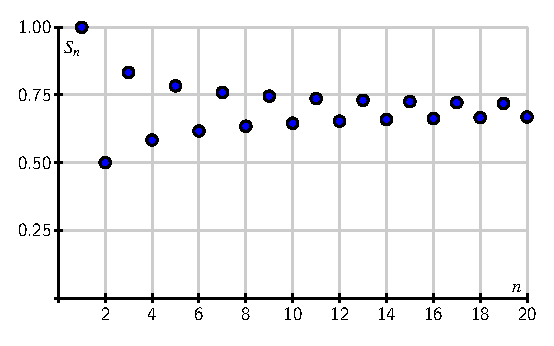
\includegraphics{figures/8_4_Alternating_Series.eps}}
%\caption{Partial sums of an alternating series}
%\label{T:8.4.1_Alternating_Series}
\end{center}
%\end{figure}
Notice that the partial sums seem to oscillate back and forth around some fixed number, getting closer to that fixed number at each successive step. So there appears to be a limit for this sequence of partial sums.


\ea
\end{activitySolution}
\aftera 